\documentclass[a4paper, 12pt]{report}


\usepackage[czech]{babel} % czech language
\usepackage{amssymb} % for math symbols
\usepackage{amsmath} % for math symbols
\usepackage{pdfpages} % for including pdf files
\usepackage{microtype} % better text rendering
\usepackage[T1]{fontenc} % better text rendering
\usepackage{graphicx} % for images
\usepackage[hidelinks]{hyperref} % for clickable links, hidelinks hides the ugly boxes
\usepackage[a4paper,width=160mm,top=25mm,bottom=25mm,bindingoffset=6mm]{geometry} % page layout
\usepackage[pagestyles]{titlesec} % for customizing chapter titles
\usepackage{parskip} % for no indent and space between paragraphs
\usepackage{enumitem} % for customizing lists
\usepackage{fancyhdr} % for customizing headers and footers
\usepackage{bm} % for bold math symbols
\usepackage{tocloft} % for customizing table of contents
\usepackage{multicol} % for multiple columns
\usepackage{textcase} % for uppercasing text
\usepackage{tikz} % for drawing
\usepackage{float} % for floating images
\usepackage{caption} % for customizing captions
\usepackage{hhline} % for double lines in tables
\usetikzlibrary{shapes.geometric} % for drawing

% toc font
\renewcommand{\cfttoctitlefont}{\normalfont\Huge\sffamily\bfseries}
\renewcommand{\cftchapfont}{\sffamily\normalsize\bfseries}
\renewcommand{\cftsecfont}{\sffamily\normalsize}



% for customizing bibliography title
\addto{\captionsczech}{\renewcommand{\bibname}{Seznam zdrojů}}

\pagestyle{fancy}
\fancyhf{}
\fancyhead[LE]{\nouppercase{\chaptername}}
\fancyhead[RO]{\nouppercase{\chaptername}}
\fancyfoot[C]{\sffamily\selectfont--~\thepage~--}
\setlength{\headheight}{15pt}
\renewcommand{\headrulewidth}{0.4pt}

\renewcommand{\sectionmark}[1]{\markright{#1}}

% for customizing chapter titles
\titleformat{\chapter}[display]{\sffamily\bfseries}{}{0pt}{\Huge}

% for customizing section titles
\titleformat{\section}{\Large\sffamily\bfseries}{\thesection}{1em}{}

% for customizing subsection titles
\titleformat{\subsection}{\large\sffamily\bfseries}{\thesubsection}{1em}{}

% for customizing subsubsection titles (no new lines after title)
\titleformat{\subsubsection}[runin]{\sffamily\bfseries}{\thesubsubsection}{1em}{}

\DeclareCaptionLabelFormat{myformat}{\sffamily#1 #2}
\captionsetup[figure]{labelformat=myformat}


\begin{document}

\begin{titlepage}
    \begin{center}
        \Huge

        % \textbf{Univerzita Jana Evangelisty Purkyně \\v Ústí nad Labem}
        \textbf{\textsf{\textls*[-50]{Univerzita Jana Evangelisty Purkyně \\v Ústí nad Labem}}}
            
        \vspace{1cm}
        \LARGE
        \textbf{\textsf{\textls*[-25]{Přírodovědecká fakulta}}}
        
        \vspace{2cm}
        \includegraphics[width=0.5\textwidth]{static/PřF-UJEP-logo.png}
        \vspace{3cm}
            
        \textbf{\textsf{\textls*[-50]{Vytváření bounding boxů ve snímcích buněk pořízených optickým mikroskopem}}}
        
        \vspace{1cm}

        \large
        BAKALÁŘSKÁ PRÁCE

        \vfill

            \begin{flushleft}
                
            \large
            \textbf{Vypracoval:} Petr Kotlan \\
            \vspace{0.3cm}
            \textbf{Vedoucí práce:} doc. RNDr. Zbyšek Posel, Ph.D. \\
            \vspace{1.5cm}
            \textbf{Studijní program:} Matematika ve firmách a veřejné správě
        \end{flushleft}

        \vspace{1.5cm}
        
        \LARGE
        Ústí nad Labem 2025

    \end{center}
\end{titlepage}

\thispagestyle{empty}
\mbox{}


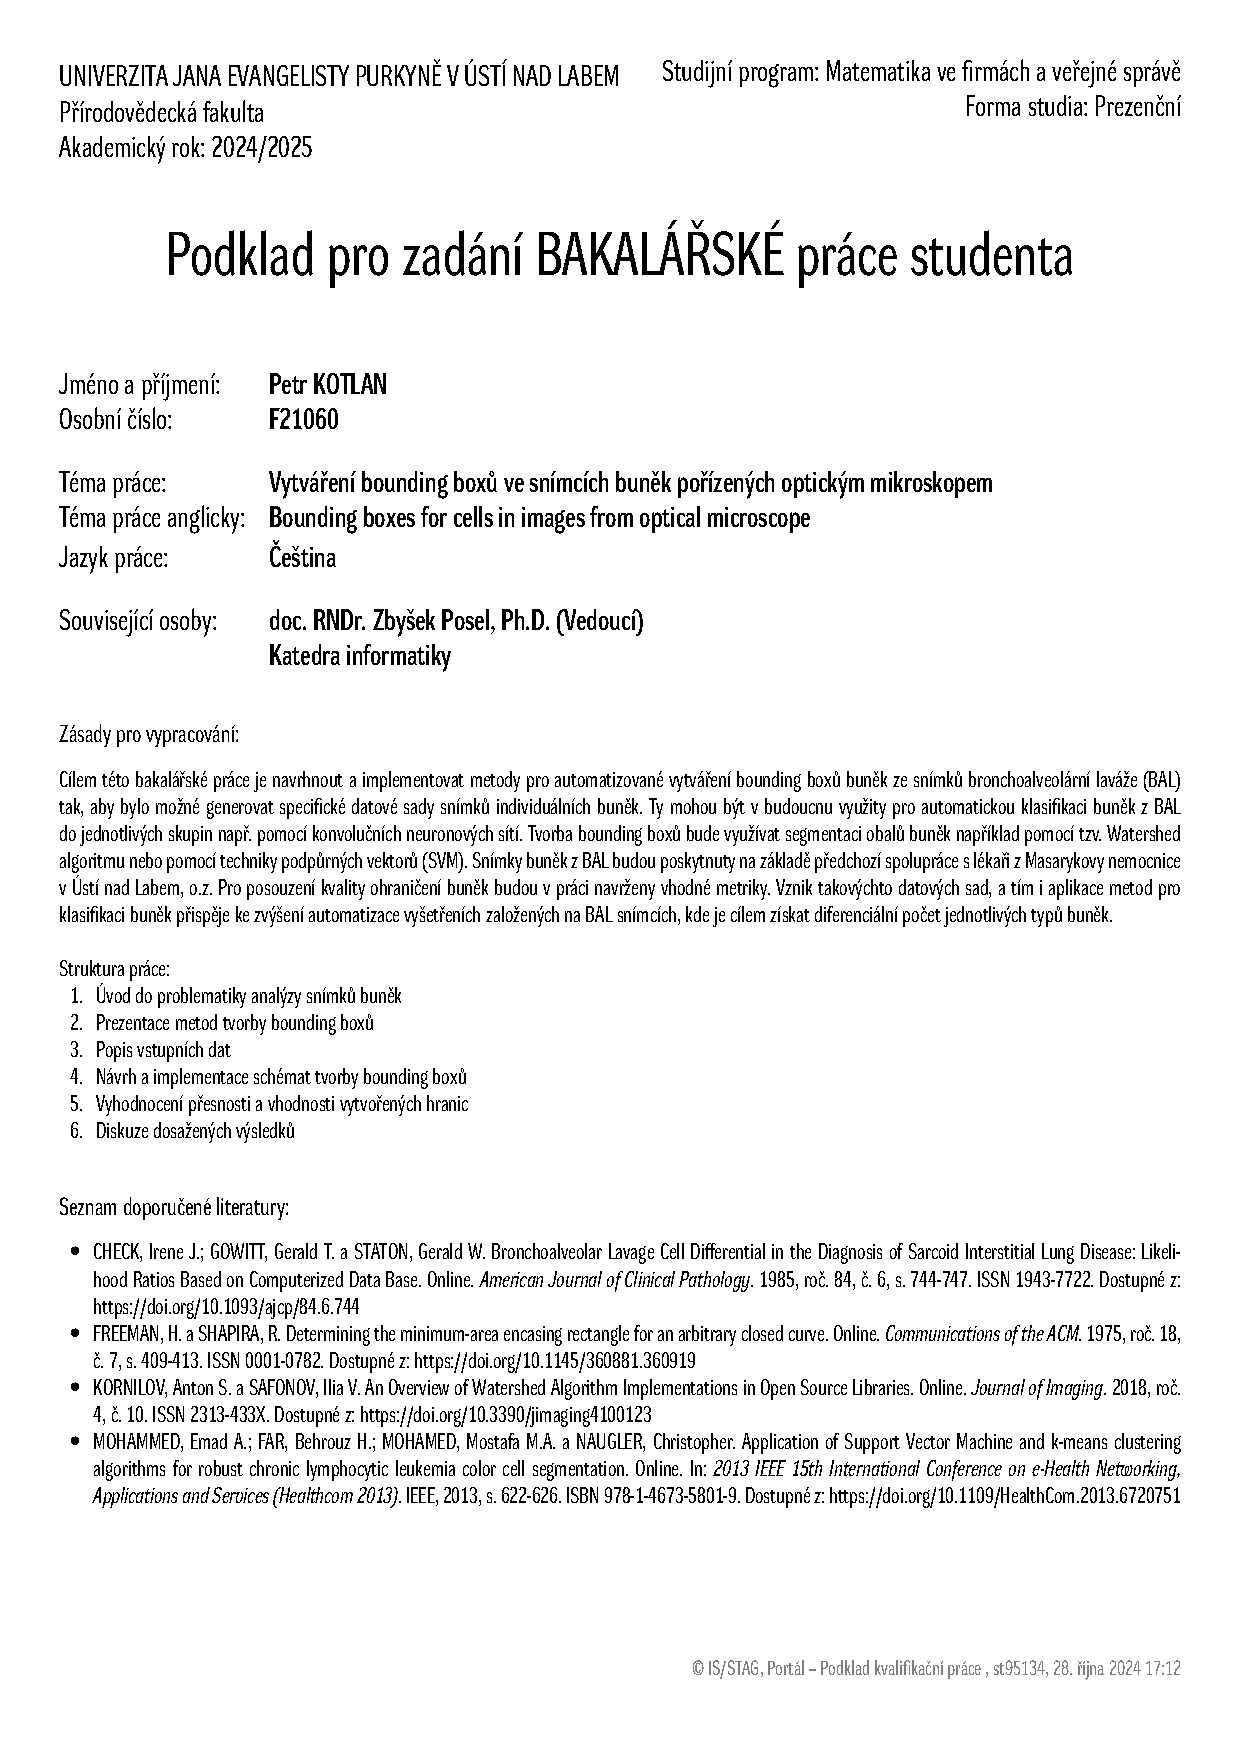
\includepdf[pages=-]{static/podklad_bp.pdf}
\thispagestyle{empty}
\addtocounter{page}{1} 

\textbf{Prohlášení}

\vspace{1cm}

Prohlašuji, že jsem tuto bakalářskou práci vypracoval samostatně a použil jen pramenů, které
cituji a uvádím v přiloženém seznamu literatury.

\vspace{0.5cm}

Byl jsem seznámen s tím, že se na moji práci vztahují práva a povinnosti vyplývající ze zákona
č. 121/2000 Sb., ve znění zákona č. 81/2005 Sb., autorský zákon, zejména se skutečností,
že Univerzita Jana Evangelisty Purkyně v Ústí nad Labem má právo na uzavření licenční
smlouvy o užití této práce jako školního díla podle § 60 odst. 1 autorského zákona, a s tím, že
pokud dojde k užití této práce mnou nebo bude poskytnuta licence o užití jinému subjektu,
je Univerzita Jana Evangelisty Purkyně v Ústí nad Labem oprávněna ode mne požadovat
přiměřený příspěvek na úhradu nákladů, které na vytvoření díla vynaložila, a to podle
okolností až do jejich skutečné výše.

\vspace{1cm}

\begin{multicols}{2}
    \begin{flushleft}
    V Ústí nad Labem dne ..............................
    \end{flushleft}

\newcolumn

\begin{flushright}
Podpis: ............................................
\end{flushright}


\end{multicols}

\newpage

\thispagestyle{empty}
\mbox{}
\newpage

\thispagestyle{empty}

% podekovani, vpravo dole
\null
\vfill

\begin{flushright}
    \textit{podekování}
\end{flushright}

\newpage

\thispagestyle{empty}
\mbox{}
\newpage

\thispagestyle{empty}

\textsc{Vytváření bounding boxů ve snímcích buněk pořízených optickým mikroskopem}

\vspace{0.5cm}

\textbf{Abstrakt}

\textbf{Klíčová slova}

\vspace{0.7cm}

\textsc{Bounding boxes for cells in images from optical microscope}

\textbf{Abstract}

\textbf{Keywords}

\newpage


\thispagestyle{empty}
\mbox{}
\newpage

\tableofcontents

\addcontentsline{toc}{chapter}{Úvod}

\newpage
\thispagestyle{empty}
\mbox{}
\newpage

uvod

\chapter{Metody předzpracování a segmentace obrazu}

V této kapitole jsou podrobněji popsány vybrané metody předzpracování a segmentaci obrazu.
Na závěr kapitoly jsou uvedeny nejpoužívanější vyhodnocovací metriky.

\section{Unsharp Masking}

Unsharp masking je metoda zpracování obrazu, která se používá zaostření obrázku.

\begin{equation}
    I_{\text{sharp}} = I_{\text{original}} + k \cdot (I_{\text{original}} - I_{\text{blurred}})
\end{equation}

$I_{\text{original}}$ je původní obrázek, $I_{\text{blurred}}$ je rozmazaný obrázek. Nejčastěji se k rozmazání používá Gaussovský filtr. $k$ je koeficient, který určuje sílu efektu \cite{gQ8rTS6z7UD6hnlM}.

Byla použita implementace z knihovny PIL [citace].

\section{Binarizace}

Metody binarizace (nebo také thresholdingu) mají za úkol nalézt prahovou hodnotu, podle které se obraz jednoznačně rozdělí na dvě třídy. Tím se oddělí pozadí od popředí.

\begin{figure}[H]
    \centering
    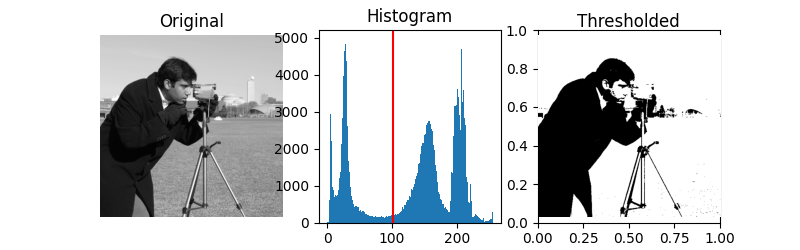
\includegraphics[width=\textwidth]{static/obrazky/thresholding_example.png}
    \caption{Binarizace obrazu Otsu metodou. Převzato z \cite{NEbfP3AWk7ALQfWN}.}
    \label{fig:thresholding}
\end{figure}

% Následuje popis několika metod binarizace.

\subsection{Otsu thresholding}

Metoda Otsu patří mezi nejpoužívanější metody binarizace. Algoritmus minimalizuje rozptyl uvnitř jednotlivých tříd.

\begin{equation}
    \sigma^2_w(t) = w_0(t)\sigma_0^2(t) + w_1(t)\sigma_1^2(t)
\end{equation}

$w_0(t)$ a $w_1(t)$ jsou pravděpodobnosti přiřazení pixelu do popředí resp. pozadí,
$\sigma_0^2(t)$ a $\sigma_1^2(t)$ jsou rozptyly tříd \cite{MopVANszPoidRZfR}.

Metoda je implementována v knihovně Scikit-image \cite{NEbfP3AWk7ALQfWN}.

\section{Morfologické operace}

Morfologické operace jsou základními nástroji pro zpracování a analýzu obrazů, které se používají k úpravě geometrických struktur v obraze. Řadí s k naprostému základu zpracování obrazu a proto zde uvedu pouze základní popis.

\subsection{Eroze}

Eroze je operace, která zmenšuje objekty v obraze. Používá se k odstranění malých objektů nebo šumu.

\subsection{Dilatace}

Dilatace je operace, která zvětšuje objekty v obraze. Používá se k vyplnění mezer nebo k propojení blízkých objektů.

\subsection{Otevření a uzavření}

Otevření je kombinace eroze a dilatace, která se používá k odstranění malých objektů a šumu. Uzavření je kombinace dilatace a eroze, která se používá k vyplnění mezer a propojení blízkých objektů.


\section{Watershed}

Algoritmus Watershed se používá k segmentaci objektů, které se dotýkají nebo překrývají.
Začne se umístěním markerů. Z každého takového bodu se pak obraz postupně „zaplavuje“, dokud se nesetkají dvě oblasti, které byly zaplavovány z různých markerů.
Nejčastěji se markery určí pomocí vzdálenostní transformace, kde se určí vzdálenost každého pixelu od nejbližšího pozadí.

\begin{figure}[H]
    \centering
    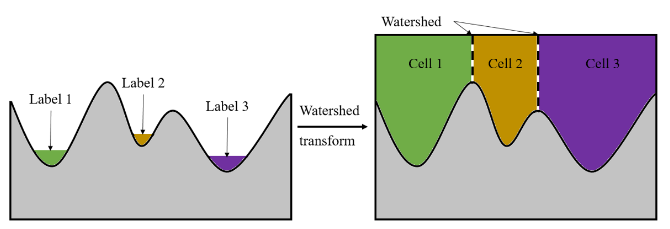
\includegraphics[width=\textwidth]{static/obrazky/watershed_process.png}
    \caption{Segmentace obrazu pomocí algoritmu Watershed. Převzato z [citace].}
    \label{fig:watershed}
    
\end{figure}
% https://www.researchgate.net/publication/349323744_Research_on_Distance_Transform_and_Neural_Network_Lidar_Information_Sampling_Classification-Based_Semantic_Segmentation_of_2D_Indoor_Room_Maps 


\section{Support Vector Machine}




\section{Vyhodnocovací metriky}

\subsection{Diceův-Sørensenův index}

Nejpoužívanější vyhdonocovací metrikou je Diceův-Sørensenův koeficient, známý též jako F1 skóre.

$$DSC = \frac{2 \times |A \cap B|}{|A| + |B|}$$

\subsection{Jaccardův index}



$$J = \frac{|A \cap B|}{|A \cup B|}$$

\chapter{Porovnání použitých metod}

\chapter{Segmentace snímků}

\section{Segmentace jader}

\tikzstyle{start} = [rectangle, rounded corners, minimum width=3cm, minimum height=1cm,text centered, draw=black, fill=blue!30]

\begin{tikzpicture}[node distance=2cm]
    \node (input) [start] {Snímek buněk};
    
\end{tikzpicture}

\section{Segmentace cytoplasmy}

\chapter{Tvorba Bounding Boxů}


\addcontentsline{toc}{chapter}{Seznam zdrojů}
\bibliographystyle{plain}
% % \bibliography{bibliografie}
\begin{thebibliography}{4}

    \bibitem{Check19851201}
    CHECK, Irene J.; GOWITT, Gerald T. a STATON, Gerald W. Bronchoalveolar Lavage Cell Differential in the Diagnosis of Sarcoid Interstitial Lung Disease: Likelihood Ratios Based on Computerized Data Base. Online. \textit{American Journal of Clinical Pathology}. 1985, roč. 84, č. 6, s.~744-747. ISSN 1943-7722. Dostupné z: \url{https://doi.org/10.1093/ajcp/84.6.744}. [cit. 2024-09-20].
    \bibitem{Freeman1975}
    FREEMAN, H. a SHAPIRA, R. Determining the minimum-area encasing rectangle for an arbitrary closed curve. Online. \textit{Communications of the ACM}. 1975, roč. 18, č. 7, s.~409-413. ISSN 0001-0782. Dostupné z: \url{https://doi.org/10.1145/360881.360919}. [cit. 2024-09-20].
    \bibitem{Kornilov2018}
    KORNILOV, Anton S. a SAFONOV, Ilia V. An Overview of Watershed Algorithm Implementations in Open Source Libraries. Online. \textit{Journal of Imaging}. 2018, roč. 4, č. 10. ISSN 2313-433X. Dostupné z: \url{https://doi.org/10.3390/jimaging4100123}. [cit. 2024-09-20].
    \bibitem{Mohammed2013}
    MOHAMMED, Emad A.; FAR, Behrouz H.; MOHAMED, Mostafa M.A. a NAUGLER, Christopher. Application of Support Vector Machine and k-means clustering algorithms for robust chronic lymphocytic leukemia color cell segmentation. Online. In: \textit{2013 IEEE 15th International Conference on e-Health Networking, Applications and Services (Healthcom 2013)}. IEEE, 2013, s.~622-626. ISBN 978-1-4673-5801-9. Dostupné z: \url{https://doi.org/10.1109/HealthCom.2013.6720751}. [cit. 2024-09-20].
    
\end{thebibliography}
\bibliography{bibliografie}
\end{document}